\documentclass{article}
\usepackage{graphicx} % Required for inserting images
\usepackage{biblatex}
\usepackage{filecontents} % Allows inline bibtex
\usepackage{array}
\usepackage{float}
\begin{filecontents}{references.bib}
@inproceedings{wang2019fast,
  author    = {Kai Wang and Don Fussell and Calvin Lin},
  title     = {Fast Fine-Grained Global Synchronization on GPUs},
  booktitle = {Proceedings of the Twenty-Fourth International Conference on Architectural Support for Programming Languages and Operating Systems (ASPLOS)},
  year      = {2019},
  pages     = {793--806},
  month     = {April},
  url       = {https://www.cs.utexas.edu/~lin/papers/asplos19.pdf}
}
\end{filecontents}

\addbibresource{references.bib}

\title{Fast, Fine-Grain GPU Synchronization Report}
\author{Siddharth Sundaram, Julian Canales, Brian Nguyen}
\date{April 28, 2025}

\begin{document}

\maketitle

\section{Introduction}
\subsection{Inspiration}

In class, we were taught that the GPU isn't fit for heavy synchronization use, which made sense considering GPU architecture. However, we came across a paper by Wang et al.~\cite{wang2019fast} that presented the idea of using fine-grain synchronization on the GPU to achieve speedup compared to fast GPU algorithms that didn't use any synchronization. We decided that it would be very interesting and rewarding to try to recreate the results from the paper, which is the motivation behind this project.

\subsection{Goals}

Initially, we sought to recreate the paper's~\cite{wang2019fast} implementation exactly, but we soon realized that would be better kept as a stretch goal. In light of this, our realistic project goals are:
\begin{itemize}
    \item Implement the basic client and server architecture discussed in the paper
    \item Measure performance on the Shared Counters mini-benchmark
    \item Measure performance on the Hash Table benchmark
    \item Measure performance on the Expectation Maximization for Gaussian Mixture Models benchmark
    \item Achieve speedup $> 1$ with our fine-grain synchronization implementation
\end{itemize}

\section{Design and Implementation}
\subsection{Design}

According to the paper, the basic implementation has client thread blocks and server thread blocks to implement efficient synchronization. Locks are initialized in the shared memory of server thread blocks to drastically decrease the latency of lock acquisitions, releases, and retries.
\\
\\
The shared data is split evenly among the server thread blocks. This way, if a client thread wants to access specific shared data, it must send a request/message to the server thread block that "owns" that data. Each server thread block has a global lock-free circular concurrent buffer (MPMC) to store client requests. Server threads are constantly trying to dequeue from the buffer, acquire the lock(s) necessary to perform the interaction with shared data (low latency due to the lock being in shared memory), perform the interaction (critical section), and release the lock(s).
\\
\\
The client thread blocks are specifically designed for a particular benchmark and execute the corresponding algorithm. Anytime a client thread wants to interact with shared data, it finds which server owns the data (usually with a modulo) and enqueues their message (operation they want done to the data) on the server's buffer. If the buffer is full, the client retries with exponential back-off.

\subsection{Implementation}

The buffer was implemented using two indices to keep track of the next index to write to and the next index to read from, as well as a \textit{bitmask} array to determine which indices contain valid data (as described in the paper). The enqueue function uses a do-while loop with atomic compare and swap (CAS) to reserve an index to write into as long as the buffer is not currently full. Once an index is successfully reserved, the message is written to that index, and the \textit{bitmask} array at that index is set to valid (1). A threadfence is used to ensure that all threads see the newly enqueued message.
\\
\\
The dequeue function also uses a do-while loop with atomic CAS to read from the buffer in a thread-safe manner. It makes sure that the buffer is not empty and that the read index contains valid data, then reads the data into a pointer and sets the index to invalid. Once again, a threadfence is used to ensure that all threads see the \textit{bitmask} change.
\\
\\
The client and server thread blocks are launched using the same kernel to ensure that they both execute at the same time. The kernel takes in the number of server blocks as a parameter and separates client and server logic with an if statement conditional on the block ID. The client threads perform the benchmark-specific algorithm, and for any part of the algorithm that interacts with shared data, the client enqueues their operation on the proper server's buffer. The client threads terminate upon termination of the algorithm. The server thread blocks immediately initialize all locks in shared memory by setting them to 0. Next, each server identifies which buffer belongs to it and begins dequeueing and servicing messages in a loop. For every message that is dequeued, the server thread acquires the proper lock(s), carries out the operation (critical section), and releases the lock(s). Once the algorithm terminates, the server threads are signaled to break out of the loop and terminate as well.

\subsection{Limitations and Roadblocks}

During development, we encountered a few difficulties:
\begin{itemize}
    \item The buffer proved to be very difficult to implement correctly while still maintaining its lock-free nature. To deal with latency that arises from contention, we used larger buffer sizes and exponential back-off, which helped but wasn't scalable.
    \item Our implementation only seems to work for some configurations of number of servers, number of clients, and buffer size. For configurations that don't work, the machine hangs indefinitely. We haven't been able to figure out the root cause for this issue.
    \item In general, complex synchronization is difficult to get working on the GPU. Even for the simple benchmark, there were initially races that were tough to detect and debug. We seemed to have fixed the races with some carefully-placed threadfences, which could have had some impact on our implementation's performance.
\end{itemize}

\section{Evaluation}

\subsection{Shared Counters}
\begin{figure}[H]
    \centering
    
    \caption{Shared Counters Speedup Graph}
    \label{fig:enter-label}
\end{figure}

For our shared counters mini-benchmark, our primary objective was to test that our fine-grain GPU implementation was working as intended (correctness). Our secondary objective was to achieve a faster runtime with our fine-grain GPU implementation than our basic GPU implementation, which used global locks to update the shared counters instead of locks in shared memory.
\\
\\
As seen in Figure 1, while our fine-grain GPU implementation was indeed faster than our basic GPU implementation, both were much worse than the sequential implementation. This is because the large majority of the execution of this benchmark was critical section work. That is, the amount of parallelism is directly capped by the number of shared counters. It would have made sense for the speedup of both implementations to increase as the number of shared counters increased, since the number of client threads was fixed and there would be less lock contention for each counter, but this is not what we observed. Perhaps our implementation would have achieved higher speedup if the benchmark did not need to synchronize so often. That being said, the shared counters benchmark served its purpose, which was to test the implementation for correctness.

\subsection{Hash Table}

For the following graphs, the number of servers only applies to the fine-grained
GPU implementation. Our sequential and basic GPU implementations do not use any 
server thread blocks, so any variances between the x-values are completely due 
to random chance. 

\begin{figure}[H]
    \centering
    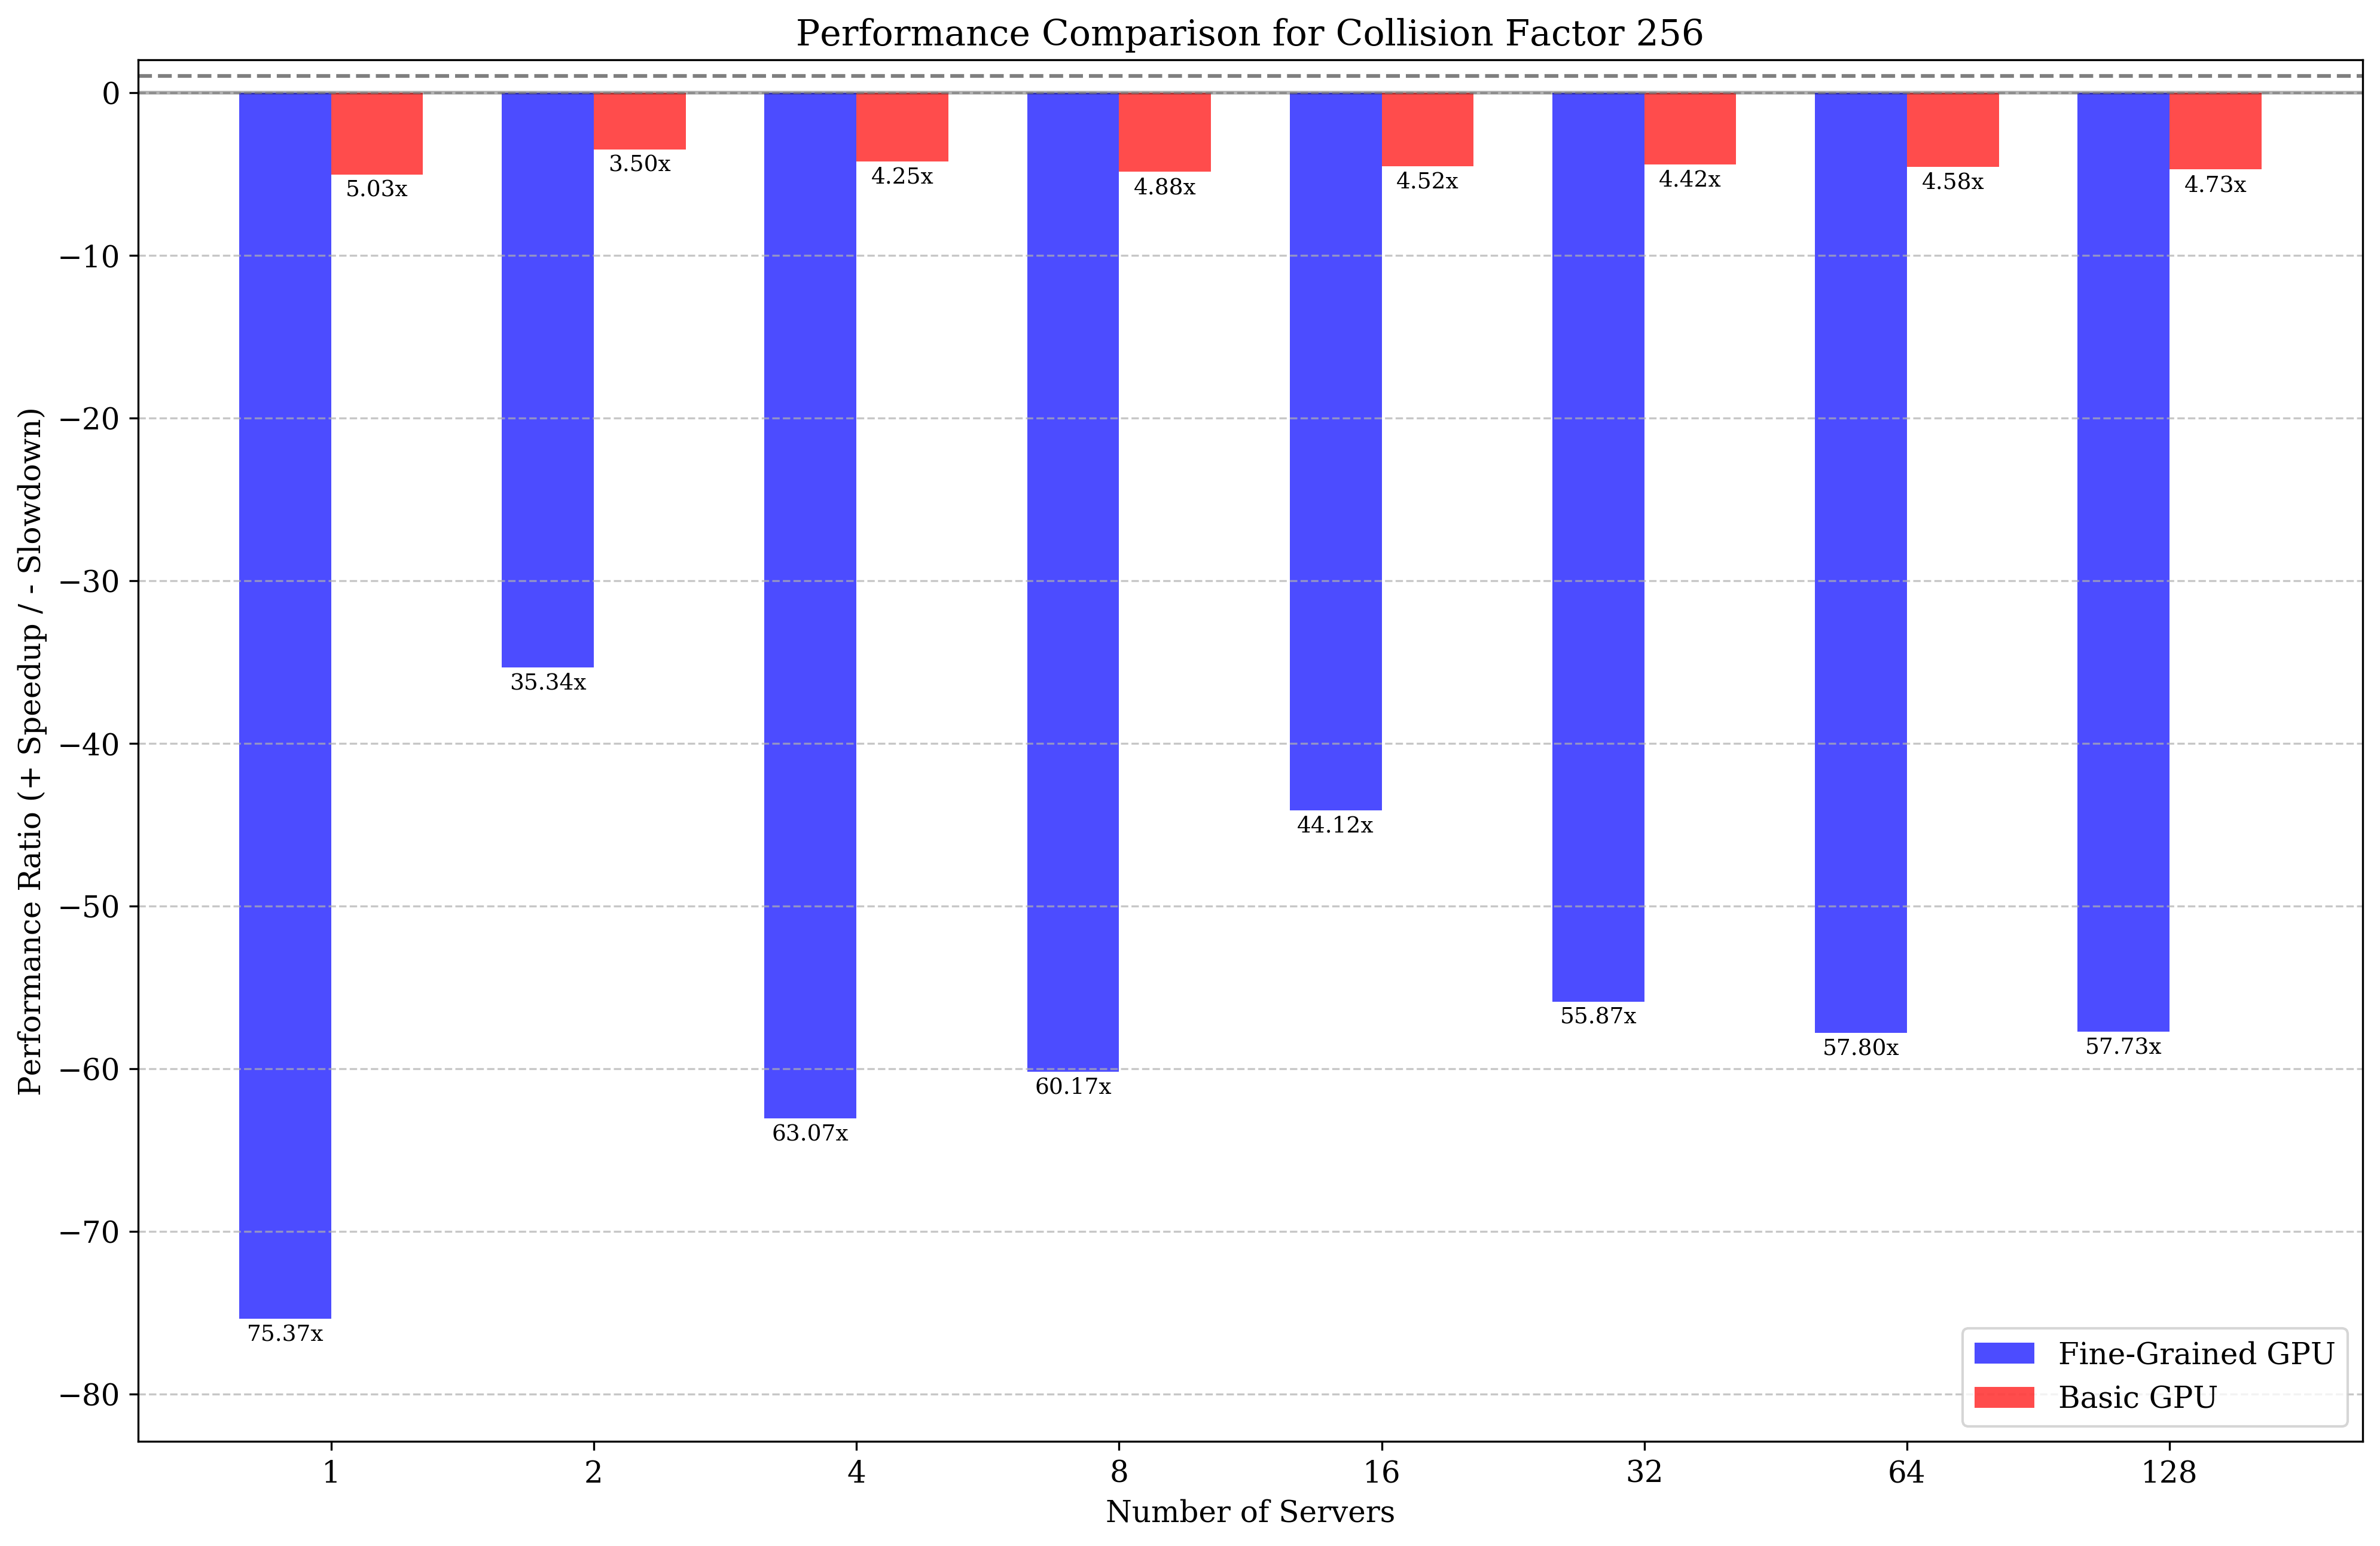
\includegraphics[width=1\linewidth]{hashtable_cf256.png}
    \caption{Hash Table Performance Graph (Collision Factor 256)}
\end{figure}

\begin{figure}[H]
    \centering
    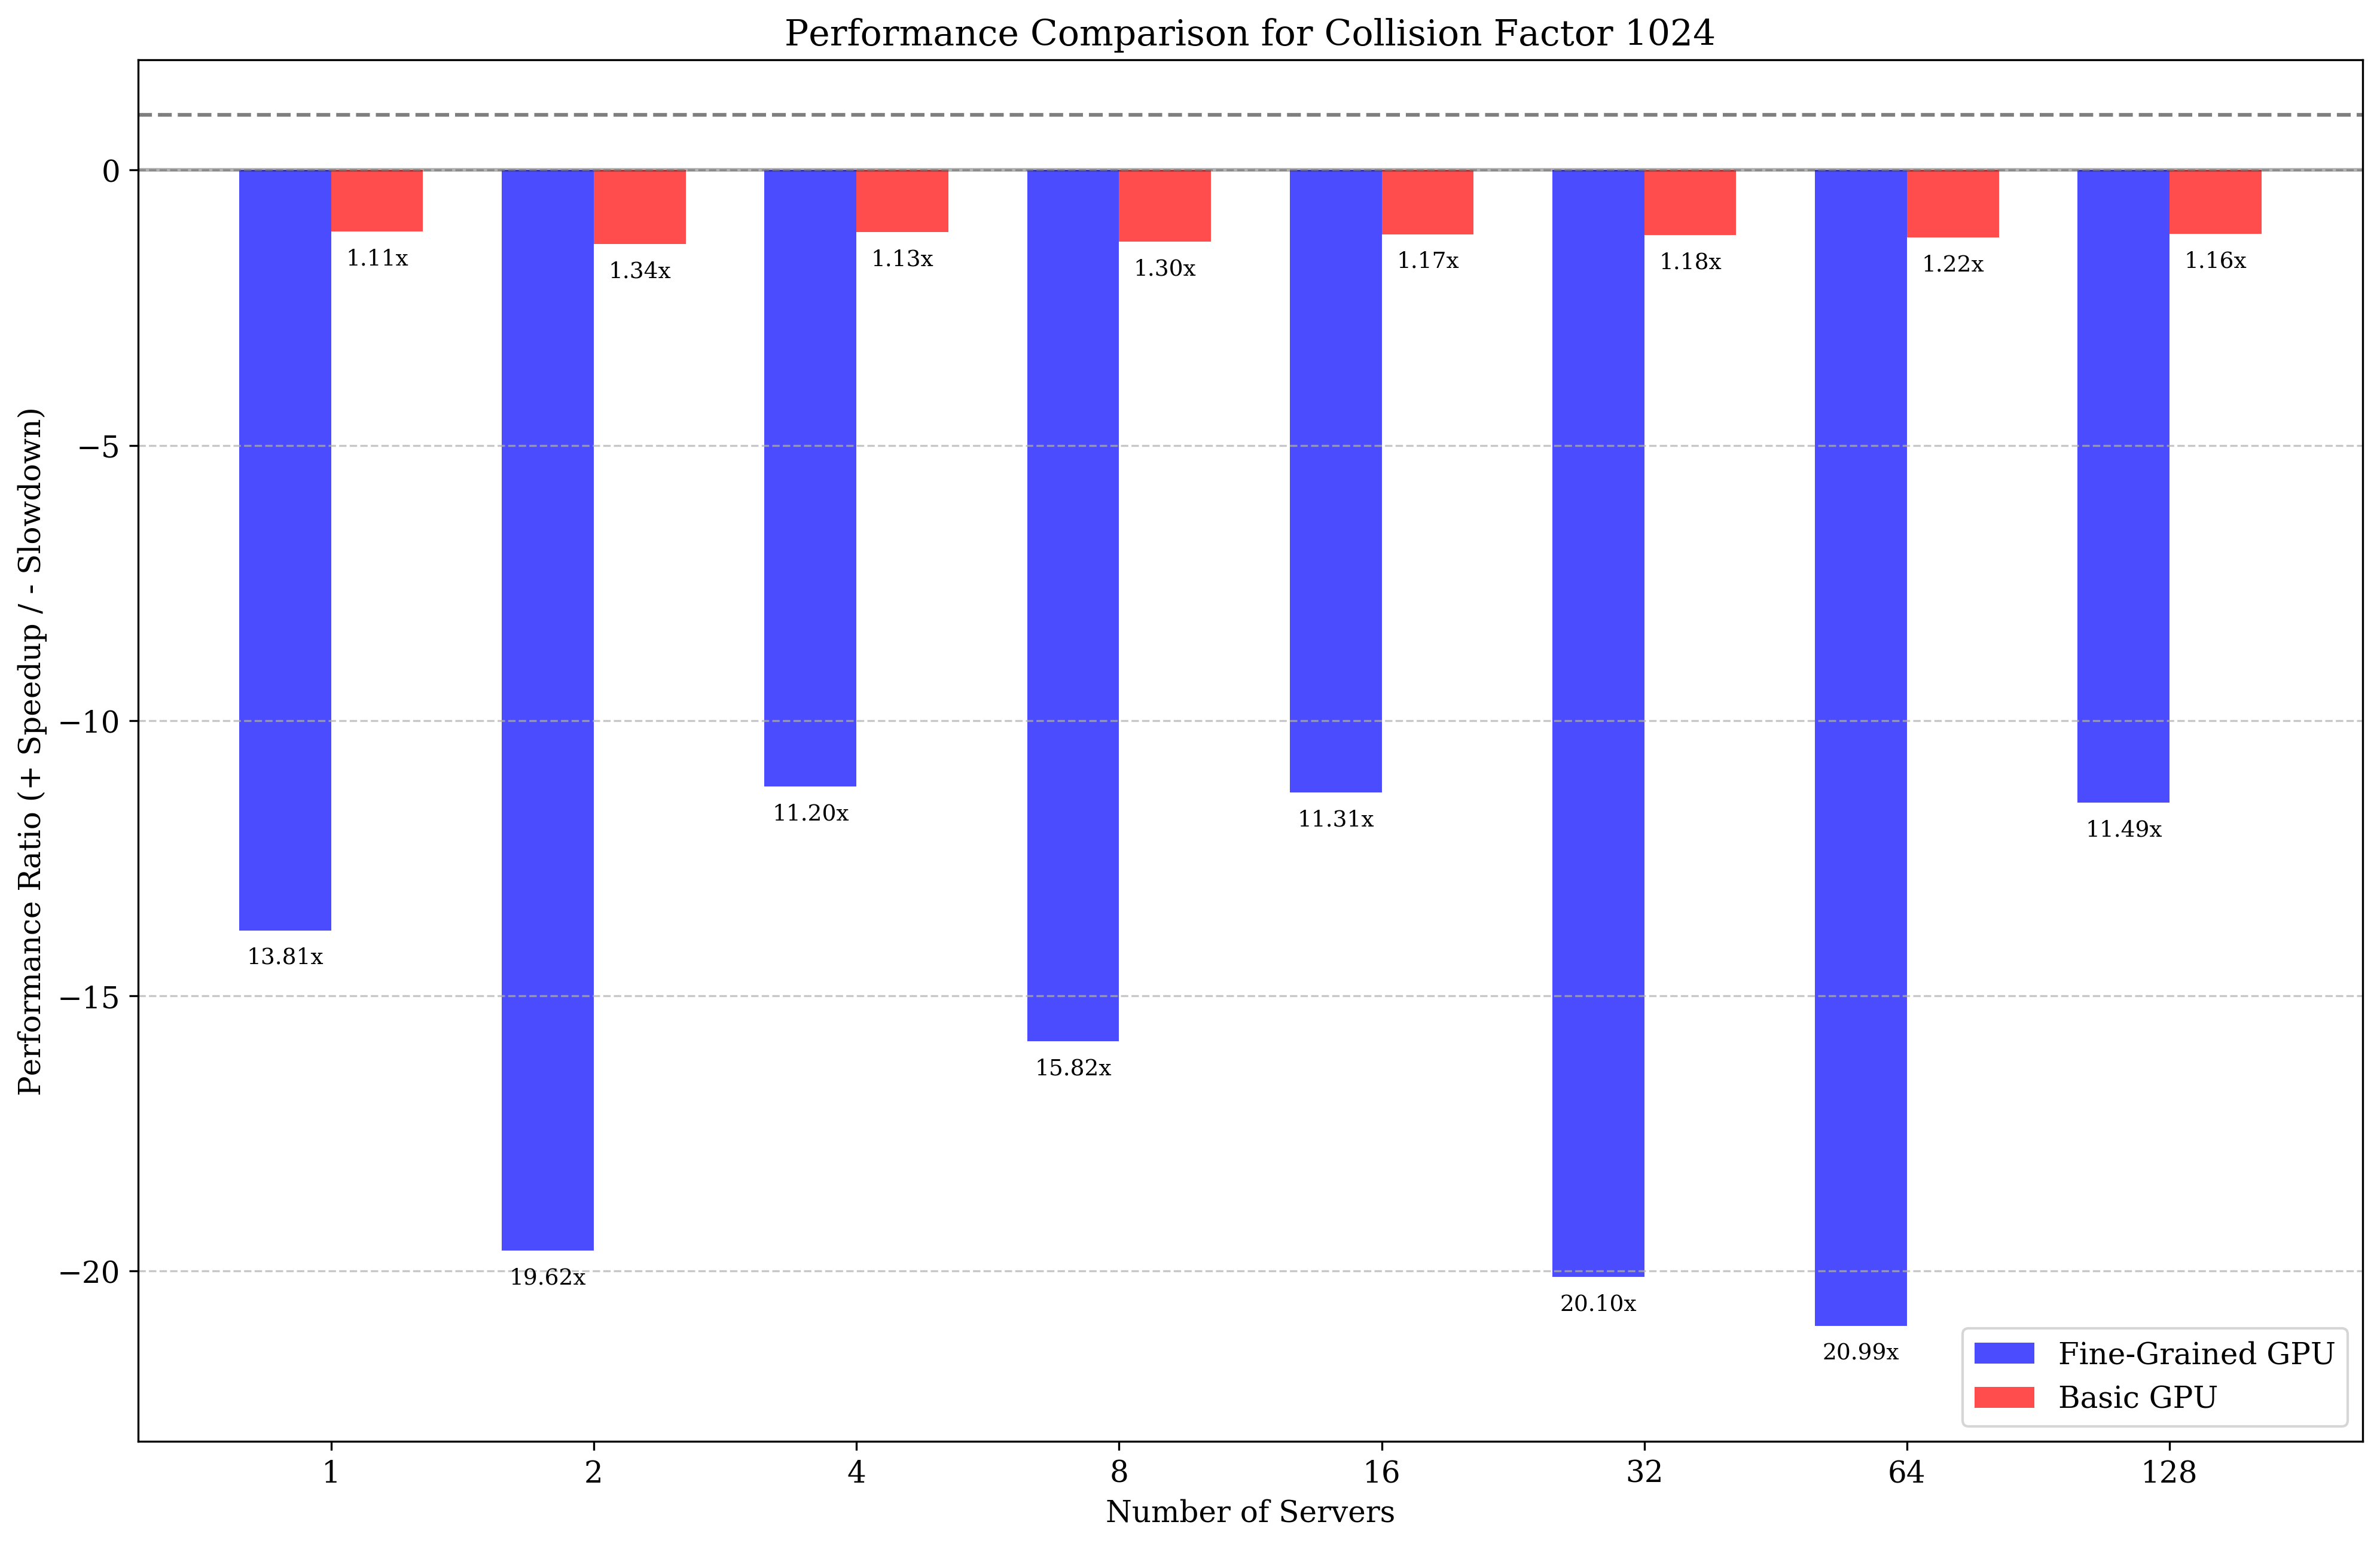
\includegraphics[width=1\linewidth]{hashtable_cf1024.png}
    \caption{Hash Table Performance Graph (Collision Factor 1024)}
\end{figure}

\begin{figure}[H]
    \centering
    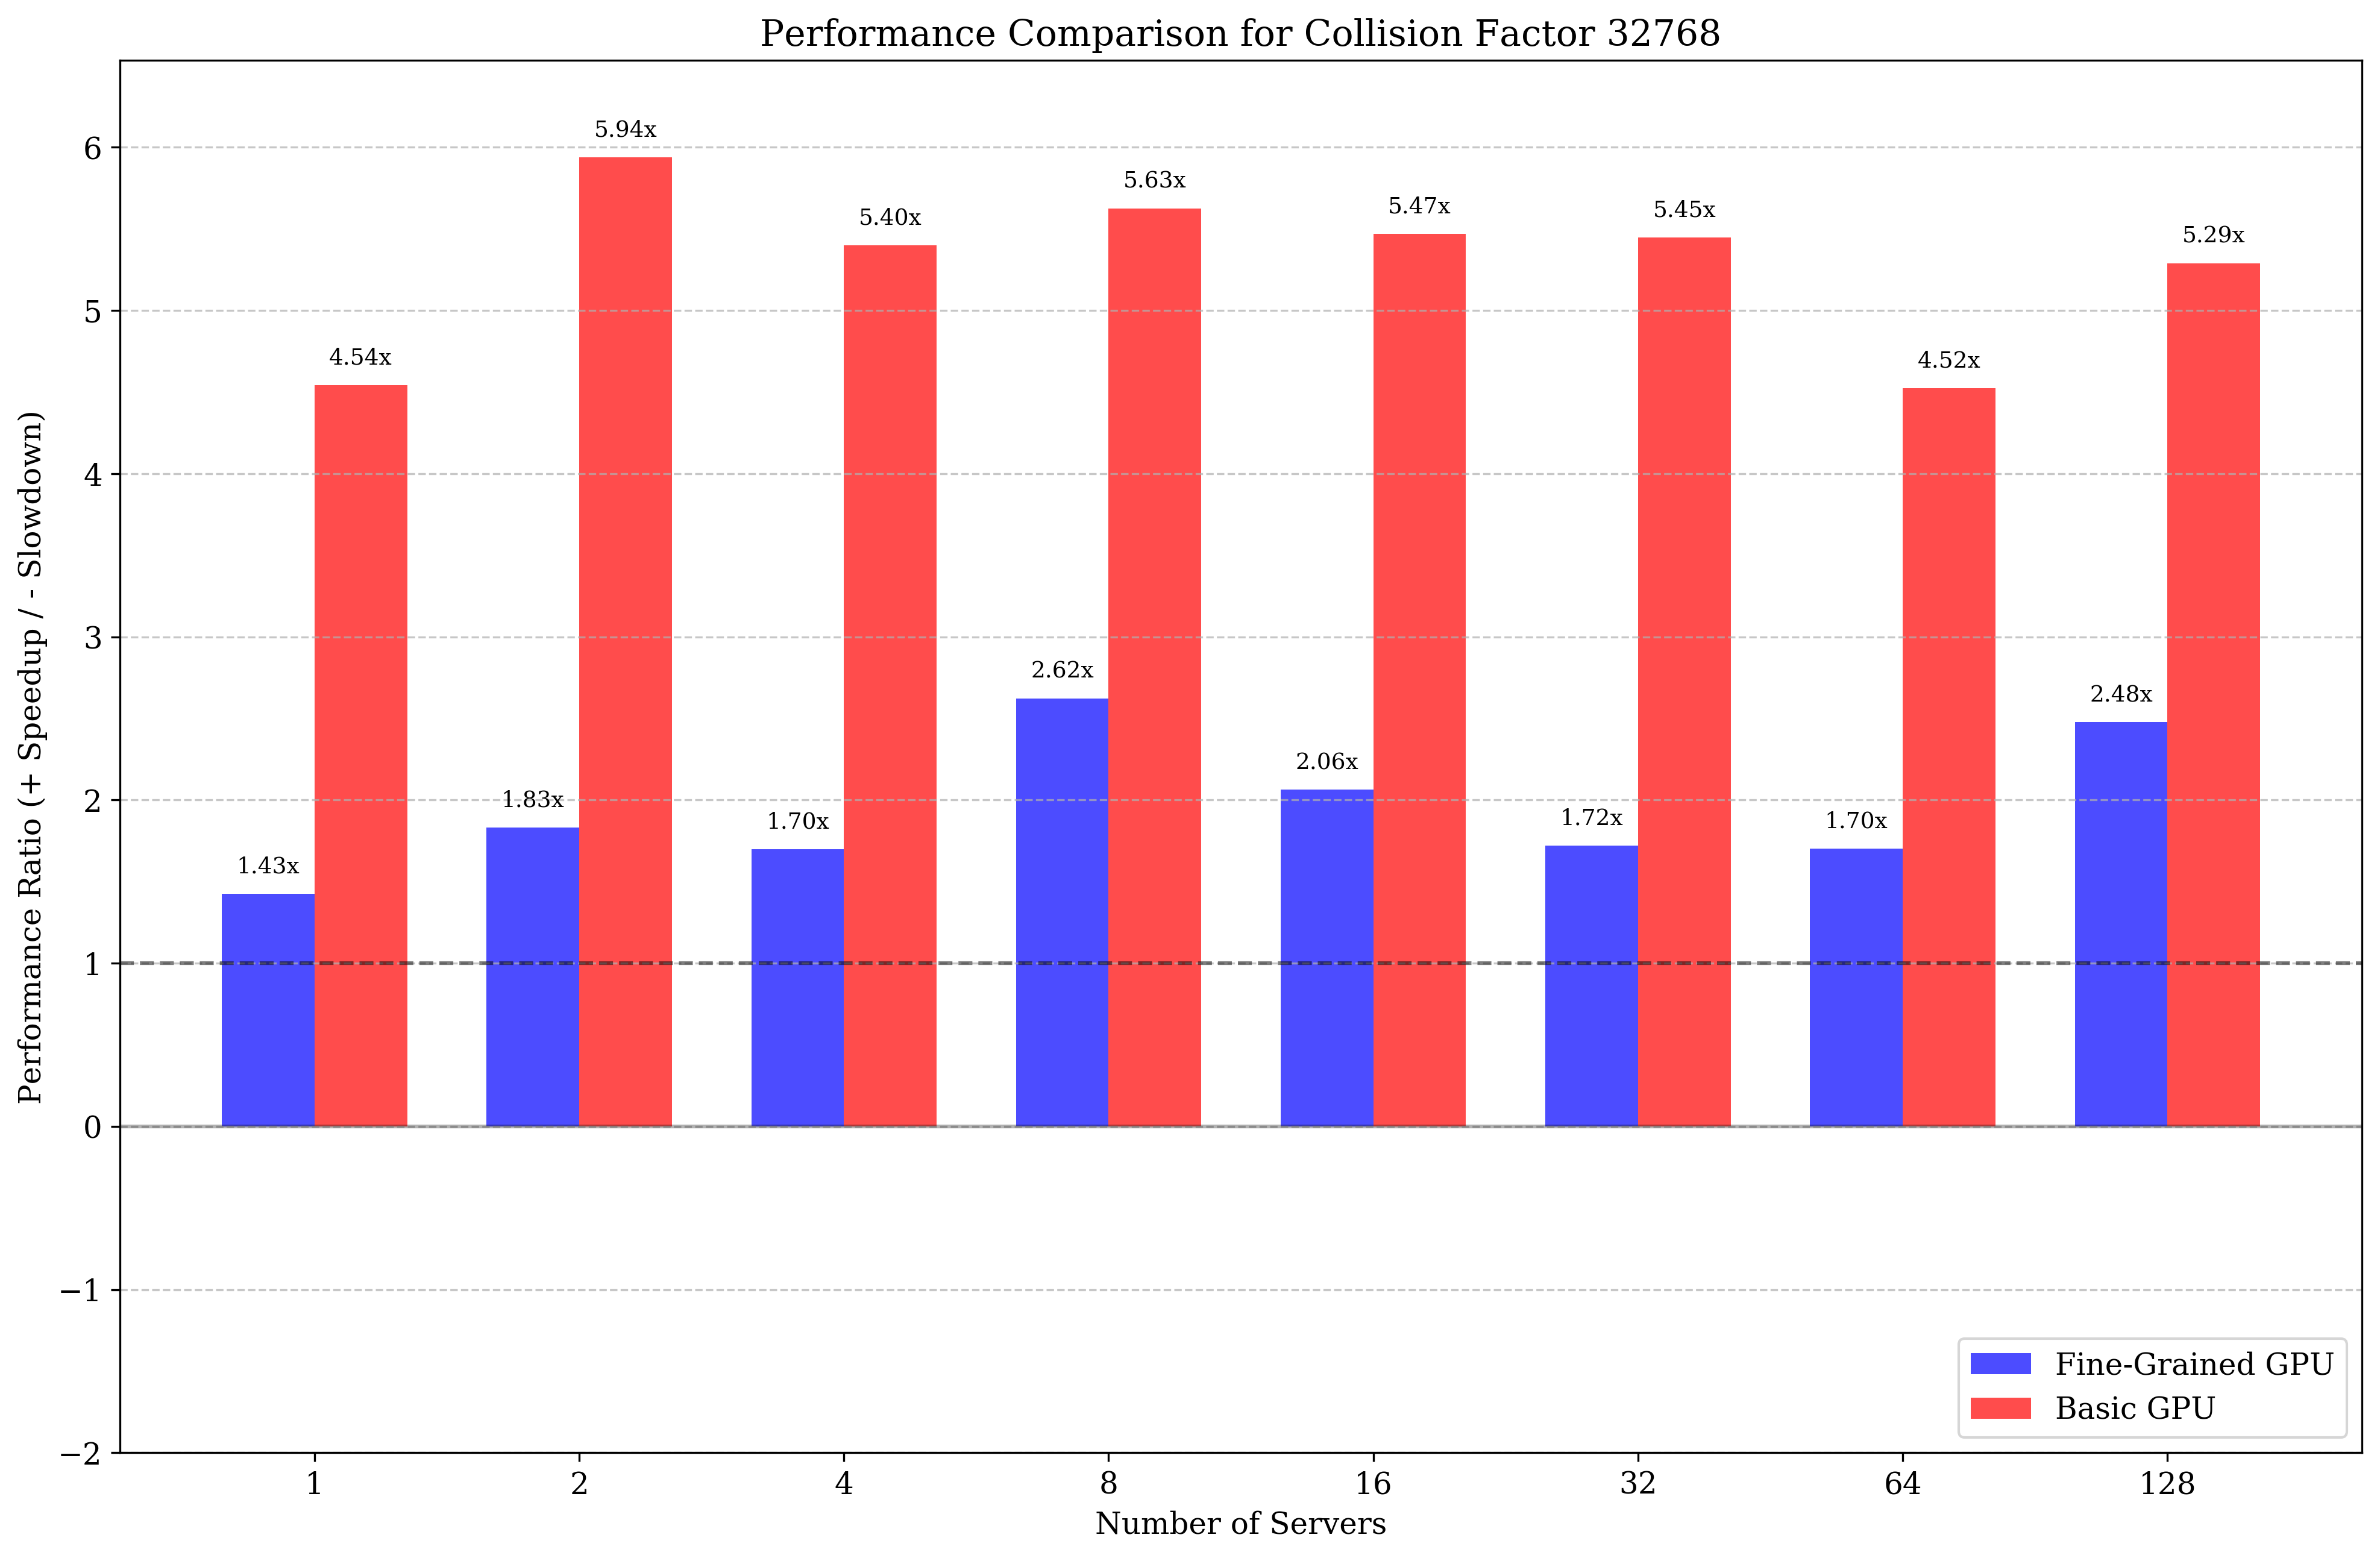
\includegraphics[width=1\linewidth]{hashtable_cf32768.png}
    \caption{Hash Table Performance Graph (Collision Factor 32768)}
\end{figure}

\begin{figure}[H]
    \centering
    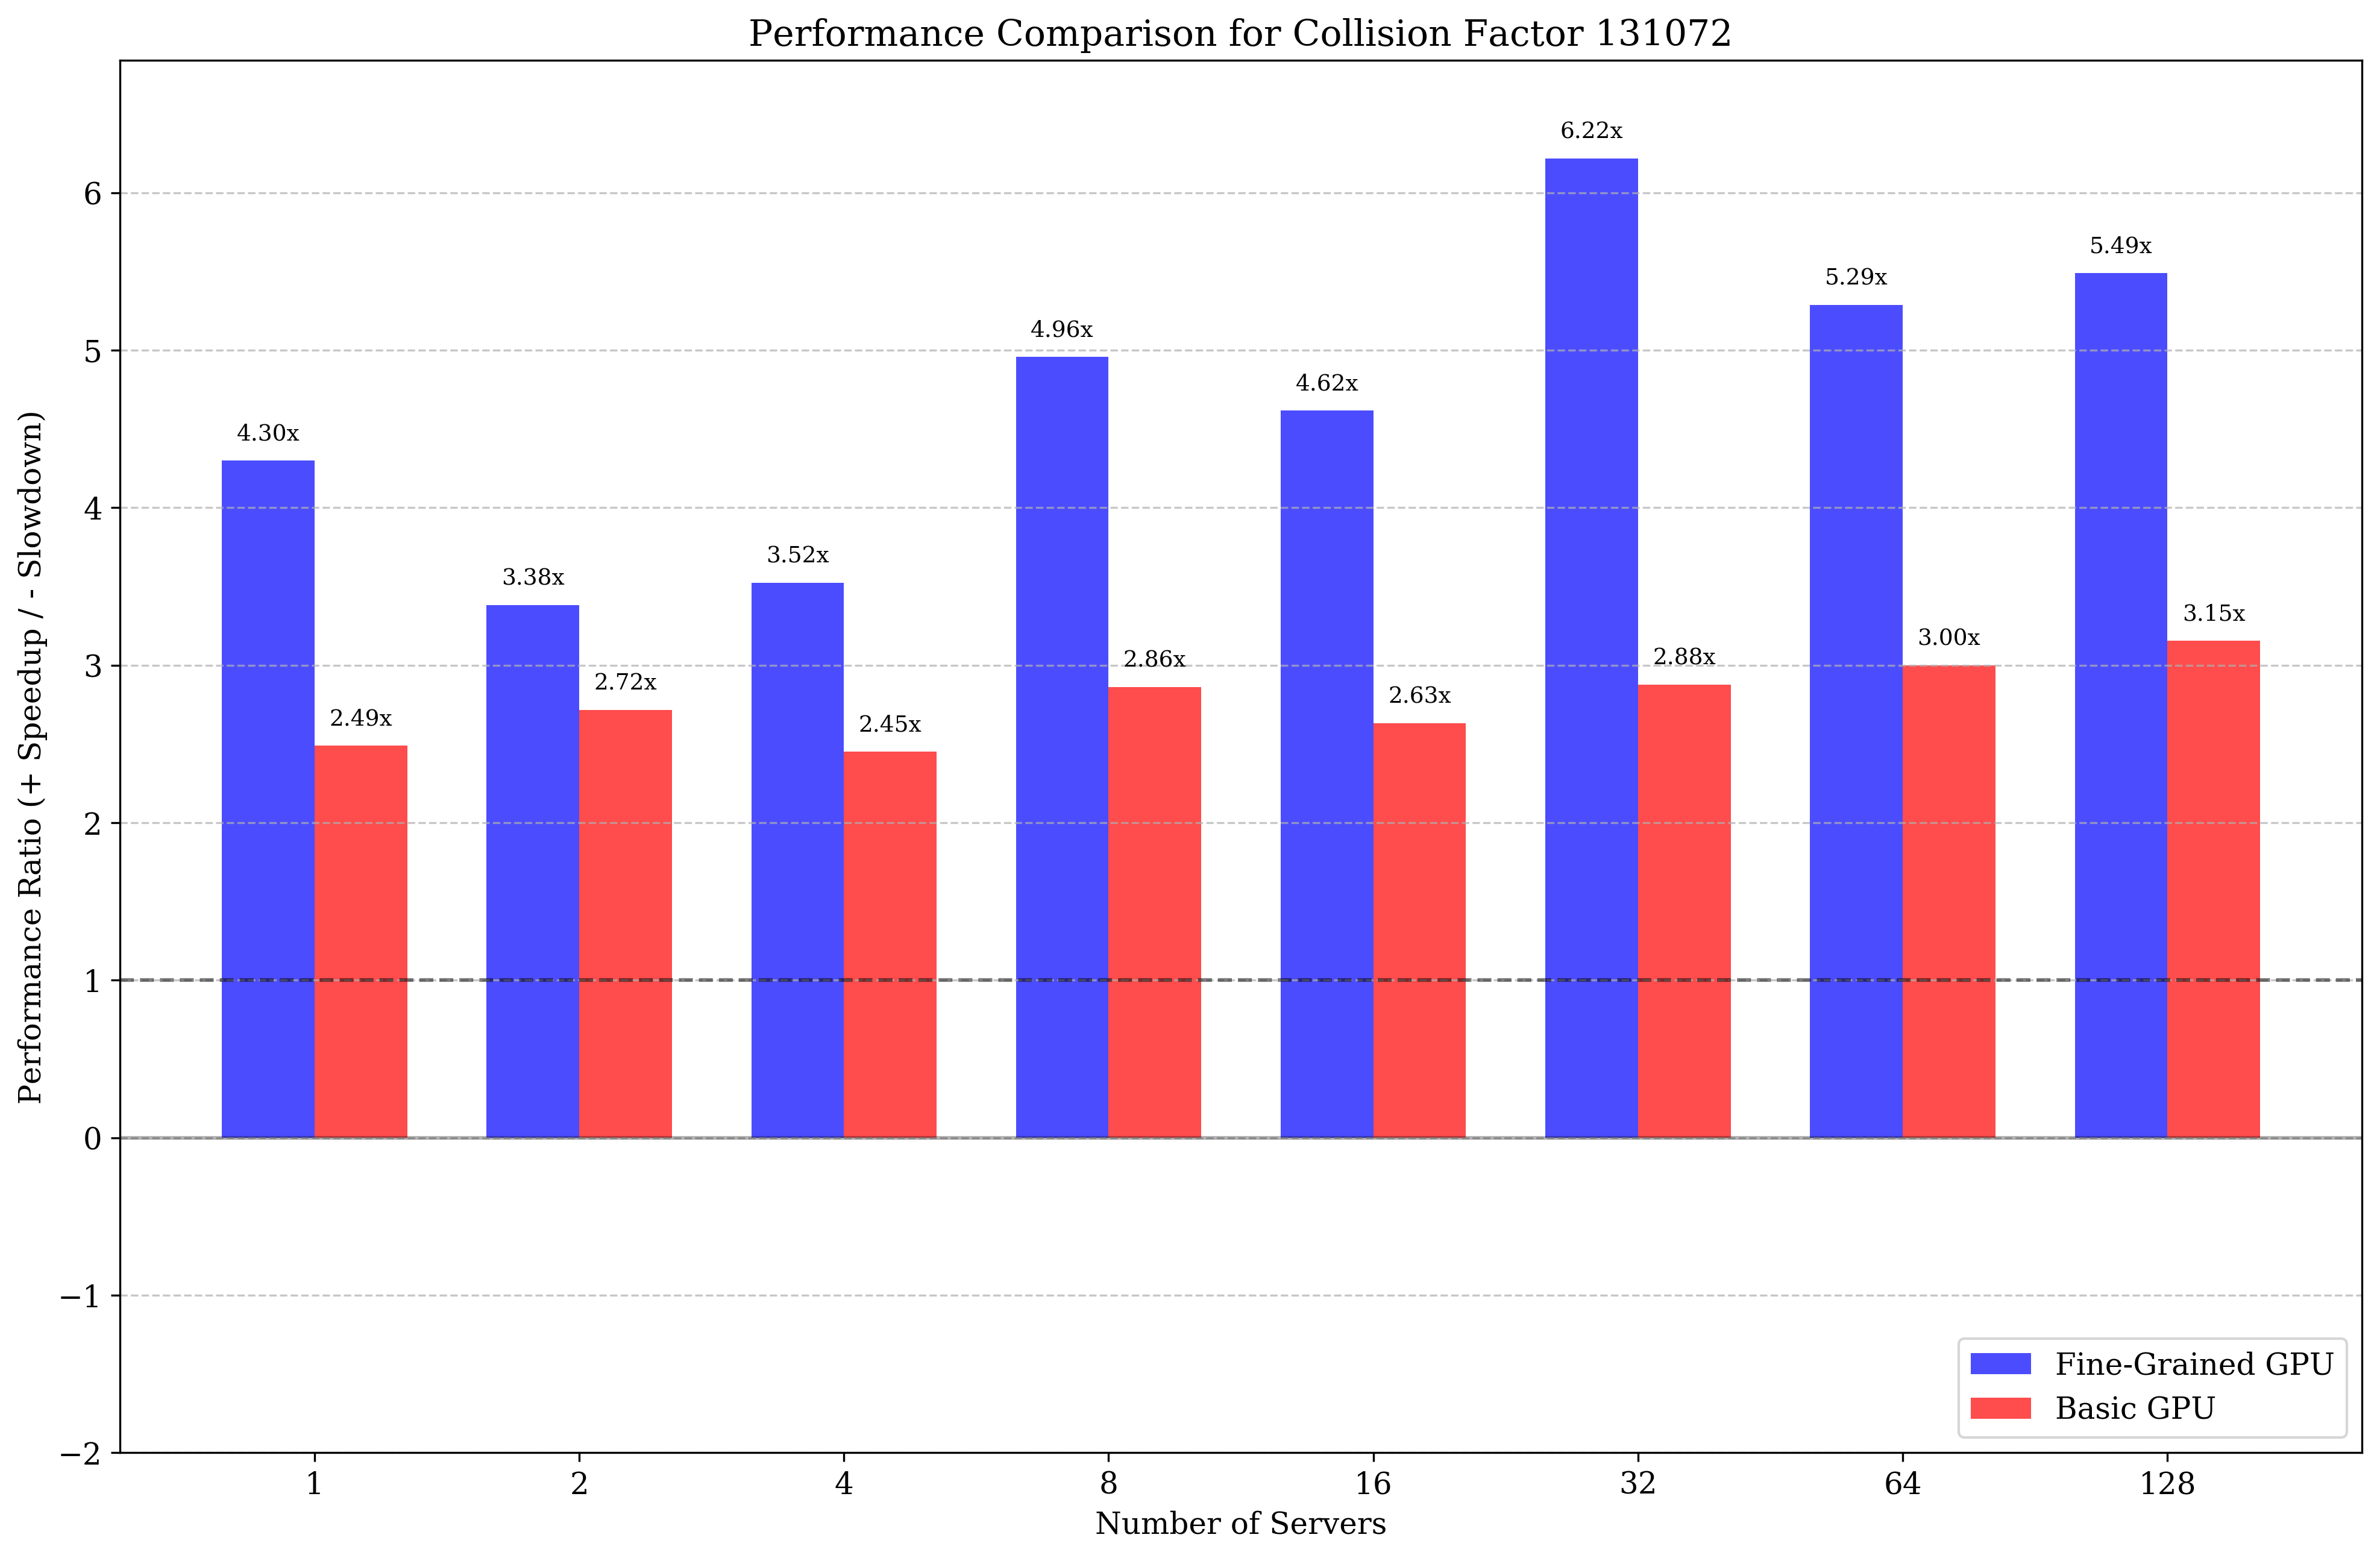
\includegraphics[width=1\linewidth]{hashtable_cf131072.png}
    \caption{Hash Table Performance Graph (Collision Factor 131072)}
\end{figure}

For our hash table benchmark, we wanted to test the performance of our fine-grain
GPU implementation on a more complex algorithm. Our goal here was to see how much 
better (or worse) it is compared to a sequential algorithm. For the actual tests,
we have threads randomly select elements from a pool to insert into the hash table.
Additionally, we made a new hash table structure for the device-side that uses
arrays of pointers, locks, and key-value pairs to store data. 
\\
\\
As a high level overview, the hash table is initialized with a certain number of
hash buckets. Each bucket is assigned a lock to prevent concurrent access, but 
can be harm performance if the number of buckets is too small. In the fine-grain
hashtable, each thread is responsible for sending exactly one request to the 
server when it wants to insert a key-value pair. The server then processes the
request, while keeping track of "empty iterations" for debugging purposes.
\\
\\
As expected, we see varying performances based on the parameter configurations
for each test we ran. We used a constant number of buckets for our hash tables
(16384), only modifying the collision factor and number of servers. We tested
a basic GPU implementation (which uses global locks) and our fine-grained 
implementation against a sequential solution. Unsurprisingly, our parallel 
runtimes are slower than sequential as a result of high lock contention and
kernel launch overhead. However, it's worth noting that the performance 
degradation is quite severe for fine-grain, especially in Figure 2, whereas the
basic GPU only suffers a little bit. With higher collision factors, we do see 
a noticeable improvement in performance. And although it looks like the number 
of servers doesn't have much of an effect on most of the tests, we do see a 
subtle upward trend in Figure 5, with the highest speedup achieved with 32
server blocks. Considering how slow the performance is for small collision 
factors, ideas for improvement could be to modify the number of buckets or 
trying to optimize lock contention between threads.

\subsection{Expectation Maximization for Gaussian Mixture Models}


\section{Conclusion}

\newpage
\printbibliography
\end{document}